\documentclass[12pt]{standalone}


\input{preamble_paper3.tex}

\begin{document}
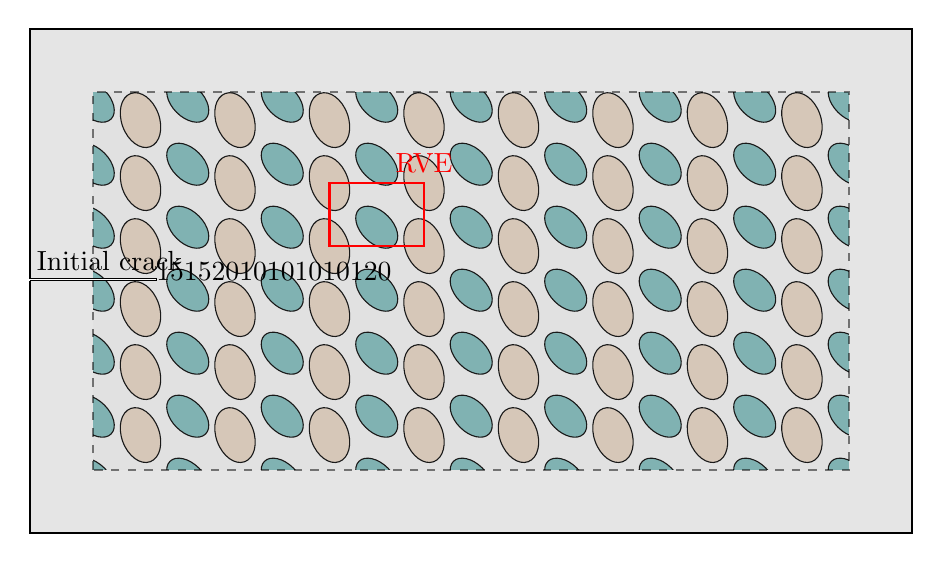
\begin{tikzpicture}[scale=0.8, text=black, draw=black]
	% matrix

	\def\h{-0.15}
	\def\hx{0.0}
	\def\hy{0.2}
	\draw[fill=gray, fill opacity=0.05, draw=none, thick] (-1, -3) rectangle (11, 3);

	\foreach \a in {-1.,0.5,...,11} {
			\foreach \b in {-3, -2,...,3} {
					\draw[fill=teal!50, rotate around={45:(\a, \b+\h)}] (\a, \b+\h) ellipse (0.25 and 0.4);
				}
		}
	\foreach \a in {-0.25,1.25,...,11} {
			\foreach \b in {-2.5, -1.5,...,3} {
					\draw[fill=brown!30, rotate around={20:(\a+\hx, \b+\h+\hy)}] (\a+\hx, \b+\h+\hy) ellipse (0.3 and 0.45);
				}
		}
	\draw[draw=none, fill=white, opacity=1] (-2, 3) rectangle (12, 4);
	\draw[draw=none, fill=white, opacity=1] (-2, -3) rectangle (12, -4.);
	\draw[draw=none, fill=white, opacity=1] (11, -3.1) rectangle (12, 3.1);
	\draw[draw=none, fill=white, opacity=1] (-2, -3.1) rectangle (-1, 3.1);
	\draw[draw=black, thick, fill=gray, fill opacity=0.2] (-2, -4) rectangle (12, 4);
	\draw[draw=black, draw opacity=0.5, thick, dashed] (-1, -3) rectangle (11, 3);

	% initial crack
	\draw[fill=white, draw=none] (-2.03, 0) rectangle (0, 0.03);
	\draw (-2.005, 0) -- (0, 0) -- (0, 0.03) -- (-2.005, 0.03);
	% \draw
	\node[anchor=south west] at (-2.05, 0) {Initial crack};

	\draw[red, thick] (2.75, 0.55) rectangle (4.25, 1.55) node[anchor=south, red] {RVE};

	% dimensions
	\dimline[label style={above, fill=none}, extension start length=0.9cm, extension end length=0.9cm] {(4.25, 3.2)}{(5.75, 3.2)}{$15$};
	\dimline[label style={above, fill=none}, extension start length=0.6cm, extension end length=0.6cm] {(2, 3.2)}{(3.5, 3.2)}{$15$};
	\dimline[label style={above, fill=none}, extension start length=0.2cm, extension end length=4.3cm] {(-2, 4.3)}{(0, 4.3)}{$20$};
	\dimline[label style={above, fill=none}, extension start length=0.cm, extension end length=0cm] {(-2, 2)}{(-1, 2)}{$10$};
	\dimline[label style={above, fill=none}, extension start length=0.cm, extension end length=0cm] {(11, 2)}{(12, 2)}{$10$};
	\dimline[label style={above, fill=none}, extension start length=0.cm, extension end length=0cm] {(10, -4)}{(10, -3)}{$10$};
	\dimline[label style={above, fill=none}, extension start length=0.cm, extension end length=0cm] {(10, 3)}{(10, 4)}{$10$};
	\dimline[label style={above, fill=none}, extension start length=0.cm, extension end length=0.2cm] {(0, 4.3)}{(12, 4.3)}{$120$};

	% \dimline[label style={above, fill=none}, extension start length=0.2cm, extension end length=0.2cm] {(-3.3, 0)}{(-3.3, 4)}{$40$};

	% \dimline[label style={below, fill=none}, extension start length=-0.5cm, extension end length=-0.5cm] {(-1.6+\hx, -1.8)}{(-0.8+\hx, -1.8)}{$x_1$};
	% \dimline[label style={above, fill=none}, extension start length=0.7cm, extension end length=0.7cm] {(-1.6+\hx-0.8, -1.2+\h+\hy)}{(-1.6+\hx-0.8, -0.4+\h+\hy)}{$x_2$};
	% \dimline[label style={above, fill=none}, extension start length=0.cm, extension end length=0.cm] {(-1.6+\hx-0.8, -0.4+\h+\hy)}{(-1.6+\hx-0.8, -0.)}{$w_1$};
	% \node at (-1.6+\hx, -0.4+\h+\hy) {\tiny $+$};
	% \node at (-1.6+\hx, -1.2+\h+\hy) {\tiny $+$};
	% \node at (-0.8+\hx, -1.2+\h+\hy) {\tiny $+$};

	% \dimline[label style={below, fill=none}, extension start length=-0.cm, extension end length=-0.9cm] {(-0.8+\hx, -1.8)}{(-0.4, -1.8)}{$x_3$};
	% \dimline[label style={above, fill=none}, extension start length=0.cm, extension end length=0.7cm] {(-1.6+\hx-0.4, -1.2+\h+\hy)}{(-1.6+\hx-0.4, -0.8+\h)}{$x_4$};

	% \node at (-0.4, -0.8+\h) {\tiny $+$};
	% \node at (-1.2, -0.8+\h) {\tiny $+$};


	% \begin{scope}[shift={(3, -5.5)}, rotate=20, scale=3]
	% 	\draw[fill=brown!30] (0, 0) ellipse (0.3 and 0.45);
	% 	\dimline[extension start length=-0.3cm, extension end length=-0.3cm] {(-0.3, -0.55)}{(0.3, -0.55)}{$x_5$};
	% 	\dimline[extension start length=0.3cm, extension end length=0.3cm] {(-0.4, -0.45)}{(-0.4, 0.45)}{$x_6$};

	% 	\draw[dashed, ] (0, 0) -- (0., 0.45) coordinate (mary);
	% 	\draw[dashed, rotate around={-20:(0, 0)}] (0, 0) -- (0.3, 0) coordinate (bob);
	% 	\coordinate (origo) at (0, 0);
	% 	\pic[draw, -latex, "$x_7$", angle eccentricity=0.5] {angle = bob--origo--mary};
	% 	\coordinate (p1) at (0, 0.24);
	% \end{scope}


	% \begin{scope}[shift={(6, -5.5)}, rotate around={45:(0, 0)}, scale=3]
	% 	\draw[fill=teal!50] (0, 0) ellipse (0.25 and 0.4);
	% 	\dimline[extension start length=-0.3cm, extension end length=-0.3cm] {(-0.25, -0.5)}{(0.25, -0.5)}{$x_8$};
	% 	\dimline[extension start length=0.3cm, extension end length=0.3cm] {(-0.35, -0.4)}{(-0.35, 0.4)}{$x_9$};

	% 	\draw[dashed] (0, 0) -- (0., 0.4) coordinate (mary);
	% 	\draw[dashed, rotate around={-45:(0, 0)}] (0, 0) -- (0.3, 0) coordinate (bob);
	% 	\coordinate (origo) at (0, 0);
	% 	\pic[draw, -latex, "$x_{10}$", angle eccentricity=0.5] {angle = bob--origo--mary};
	% \end{scope}




\end{tikzpicture}

\end{document}
